\documentclass[xcolor={usenames,dvipsnames}]{beamer}
\usepackage[utf8]{inputenc}
\usepackage{tikz}
\usetikzlibrary{arrows.meta}
\tikzset{>={Latex[width=2mm,length=2mm]},
  base/.style = {
    rectangle, rounded corners, draw=black,
    minimum height=1cm, text centered, font=\sffamily
  },
  process/.style = {
    base, minimum width=2.5cm, fill=orange!15,
    font=\ttfamily
  },
}

\usepackage[normalem]{ulem}

\graphicspath{{./img/},{../2021_05/img/},{../2020_03/img/}}
\DeclareGraphicsExtensions{.png,.jpg,.pdf}

\usepackage{hyperref}
\hypersetup{colorlinks,urlcolor=blue!50!black,linkcolor=red}

\usepackage{fontawesome}
\usepackage{listings}

\title{\small Máster en Sistemas Electrónicos Avanzados (MSEA)\\\Large Co-simulación y verificación funcional con\\VHDL, C/C++ y Python/m\\{\small $\{$cosim$\}$}}
\author{Unai Martinez Corral\\\href{mailto:unai.martinezcorral@ehu.eus}{\faEnvelope~unai.martinezcorral@ehu.eus}\\\href{https://orcid.org/0000-0003-1752-9181}{\faGlobe~ORCID} ~\href{https://github.com/umarcor}{\faGithub~umarcor} ~\href{https://gitlab.com/umarcor}{\faGitlab~umarcor}}
\institute{Escuela de Ingeniería de Bilbao\\Universidad del País Vasco/Euskal Herriko Unibertsitatea (UPV/EHU)}
\date{2022/05}

\begin{document}

\frame{\titlepage}

\begin{frame}
\frametitle{VHDL co-simulation with GHDL}
\begin{center}
\begin{minipage}{.4\linewidth}
\href{https://ghdl.github.io/ghdl-cosim}{\includegraphics[width=.9\linewidth]{ghdlcosim_logo}}
\end{minipage}
\begin{minipage}{.45\linewidth}
\href{https://ghdl.github.io/ghdl-cosim}{\faBook~ghdl.github.io/ghdl-cosim}
\end{minipage}
\end{center}

\vfill

\footnotesize

\begin{itemize}
\item Indirect co-simulation:
  \begin{itemize}
    \item {\color{OliveGreen} Partial} Verilog Procedural Interface (\textbf{VPI}),
    {\color{gray} also known as Program Language Interface (\textbf{PLI}) 2.0}.

    \item \sout{VHDL Procedural Interface (\textbf{VHPI})}.

      {\color{OliveGreen}
        There is AVHPI \href{https://ghdl.github.io/ghdl-cosim/vhpidirect/grt.html}{\faBook}, and work in progress by
        Marlon James for adding VHPI support.
      }
  \end{itemize}

\vfill

\item Direct co-simulation:
\begin{itemize}
  \item Specific implementations of (a draft of) VHPIDIRECT, \sout{such as Foreign Language Interface (\textbf{FLI}) or
  Xilinx Simulation Interface (\textbf{XSI})}.
  \item \sout{Direct Programming Interface (\textbf{DPI})}.

  {\color{OliveGreen} The VASG expects to standardize a direct interface (VHDPI or VHFFI) in the next revision of the standard (202X).}
\end{itemize}

\end{itemize}
\vfill
\end{frame}

\begin{frame}
\frametitle{Direct VHDL co-simulation with GHDL}

\begin{itemize}
\item Type declarations \href{https://ghdl.github.io/ghdl-cosim/vhpidirect/declarations.html}{\faBook}
\item Linking object files \href{https://ghdl.github.io/ghdl-cosim/vhpidirect/linking.html}{\faBook}
\item Notebook: Common mistakes \href{https://ghdl.github.io/ghdl-cosim/vhpidirect/notebook/mistakes.html}{\faBook}
\end{itemize}

\vfill

Exercises:
\begin{itemize}
\item 'rand' from stdlib
\href{https://ghdl.github.io/ghdl-cosim/vhpidirect/examples/quickstart.html\#rand-from-stdlib}{\faBook}
\href{https://github.com/ghdl/ghdl-cosim/blob/master/vhpidirect/quickstart/random}{\faCode}

\item 'sin' from libmath
\href{https://ghdl.github.io/ghdl-cosim/vhpidirect/examples/quickstart.html\#sin-from-libmath}{\faBook}
\href{https://github.com/ghdl/ghdl-cosim/blob/master/vhpidirect/quickstart/math}{\faCode}

\item custom C
\href{https://ghdl.github.io/ghdl-cosim/vhpidirect/examples/quickstart.html\#custom-c}{\faBook}
\href{https://github.com/ghdl/ghdl-cosim/blob/master/vhpidirect/quickstart/customc}{\faCode}
\end{itemize}

\end{frame}

\begin{frame}
\frametitle{Direct co-simulation with GHDL: wrapping}

\begin{itemize}
\item Wrapping a simulation \href{https://ghdl.github.io/ghdl-cosim/vhpidirect/wrapping.html}{\faBook}
\item How to use GHDL from an external C program? \href{https://ghdl.github.io/ghdl-cosim/vhpidirect/notebook/howtouseghdlfromc.html}{\faBook}
\end{itemize}

\vfill

Exercises:
\begin{itemize}
\item basic
\href{https://ghdl.github.io/ghdl-cosim/vhpidirect/examples/quickstart.html\#basic}{\faBook}
\href{https://github.com/ghdl/ghdl-cosim/blob/master/vhpidirect/quickstart/wrapping/basic}{\faCode}

\item time
\href{https://ghdl.github.io/ghdl-cosim/vhpidirect/examples/quickstart.html\#time}{\faBook}
\href{https://github.com/ghdl/ghdl-cosim/blob/master/vhpidirect/quickstart/wrapping/time}{\faCode}

\item exitcb
\href{https://ghdl.github.io/ghdl-cosim/vhpidirect/examples/quickstart.html\#exitcb}{\faBook}
\href{https://github.com/ghdl/ghdl-cosim/blob/master/vhpidirect/quickstart/wrapping/exitcb}{\faCode}

\item Command-Line Arguments
\href{https://ghdl.github.io/ghdl-cosim/vhpidirect/examples/quickstart.html\#command-line-arguments}{\faBook}
\href{https://github.com/ghdl/ghdl-cosim/blob/master/vhpidirect/quickstart/cli}{\faCode}

\item Setting parameters in C through VHDL generics
\href{https://ghdl.github.io/ghdl-cosim/vhpidirect/examples/quickstart.html\#setting-parameters-in-c-through-vhdl-generics}{\faBook}
\href{https://github.com/ghdl/ghdl-cosim/blob/master/vhpidirect/quickstart/cli/fcngen}{\faCode}
\end{itemize}
\end{frame}

\begin{frame}
\frametitle{Direct co-simulation with GHDL: arrays and matrices}

\begin{itemize}
\item Constrained/bounded integer arrays \href{https://ghdl.github.io/ghdl-cosim/vhpidirect/examples/arrays.html\#constrained-bounded-integer-arrays}{\faBook}
\item Constrained multidimensional arrays of doubles/reals \href{https://ghdl.github.io/ghdl-cosim/vhpidirect/examples/arrays.html\#constrained-multidimensional-arrays-of-doubles-reals}{\faBook}
\end{itemize}

\vfill

Exercises:
\begin{itemize}
\item Vector of \lstinline{std_logic}
\href{https://ghdl.github.io/ghdl-cosim/vhpidirect/examples/arrays.html\#vector-of-std-logic}{\faBook}
\href{https://github.com/ghdl/ghdl-cosim/blob/master/vhpidirect/arrays/logicvector}{\faCode}

\item Array and AXI4 Stream Verification Components
\href{https://ghdl.github.io/ghdl-cosim/vhpidirect/examples/arrays.html\#array-and-axi4-stream-verification-components}{\faBook}
\href{https://github.com/ghdl/ghdl-cosim/blob/master/vhpidirect/arrays/matrices/vunit_axis_vcs}{\faCode}

\end{itemize}
\end{frame}

\begin{frame}
\frametitle{Direct co-simulation with GHDL: shared/dynamic loading}

\begin{itemize}
\item Dynamic loading \href{https://ghdl.github.io/ghdl-cosim/vhpidirect/dynamic.html}{\faBook}
\end{itemize}

\vfill

Exercises:
\begin{itemize}
\item shlib
\href{https://ghdl.github.io/ghdl-cosim/vhpidirect/examples/shared.html\#shlib}{\faBook}
\href{https://github.com/ghdl/ghdl-cosim/blob/master/vhpidirect/shared/shlib}{\faCode}

\item dlopen
\href{https://ghdl.github.io/ghdl-cosim/vhpidirect/examples/shared.html\#dlopen}{\faBook}
\href{https://github.com/ghdl/ghdl-cosim/blob/master/vhpidirect/shared/dlopen}{\faCode}

\item shghdl
\href{https://ghdl.github.io/ghdl-cosim/vhpidirect/examples/shared.html\#shghdl}{\faBook}
\href{https://github.com/ghdl/ghdl-cosim/blob/master/vhpidirect/shared/shghdl}{\faCode}

\item py
\href{https://ghdl.github.io/ghdl-cosim/vhpidirect/examples/shared.html\#py}{\faBook}
\href{https://github.com/ghdl/ghdl-cosim/blob/master/vhpidirect/shared/py}{\faCode}

\item py/vunit
\href{https://ghdl.github.io/ghdl-cosim/vhpidirect/examples/shared.html\#py-vunit}{\faBook}
\href{https://github.com/ghdl/ghdl-cosim/blob/master/vhpidirect/shared/py/vunit}{\faCode}

\item pycb
\href{https://ghdl.github.io/ghdl-cosim/vhpidirect/examples/shared.html\#pycb}{\faBook}
\href{https://github.com/ghdl/ghdl-cosim/blob/master/vhpidirect/shared/pycb}{\faCode}

\end{itemize}
\end{frame}

\begin{frame}
  \frametitle{VUnit's external API}
  \begin{itemize}
  \item VUnit External VHDL API \href{http://vunit.github.io/data_types/user_guide.html\#external-vhdl-api}{\faBook}
  \item VUnit/cosim \href{https://vunit.github.io/cosim}{\faBook}
  \end{itemize}
  \vfill
  \begin{minipage}{.3\linewidth}
  Exercises:
  \begin{itemize}
    \item copy
    \href{https://vunit.github.io/cosim/examples/copy.html}{\faBook}
    \href{https://github.com/VUnit/cosim/tree/master/examples/copy}{\faCode}
    \item buffer
    \href{https://vunit.github.io/cosim/examples/buffer.html}{\faBook}
    \href{https://github.com/VUnit/cosim/tree/master/examples/buffer}{\faCode}
  \end{itemize}
  \end{minipage}
  \begin{minipage}{.65\linewidth}
  \includegraphics[width=\linewidth]{vunit_axiscosim.pdf}
  \end{minipage}
\end{frame}

\begin{frame}
\frametitle{Standard Direct VHDL interface proposal (VHDPI/VHFFI) }

The VHDL Analysis and Standardization Group (VASG) is working towards defining a direct co-simulation interface in the
next revision of the standard.
The interface is inspired on GHDL's direct interface, FLI, XSI and System Verilog's DPI.
In fact, one of the original motivations is allowing standardized VHDL and System Verilog co-simulation.

\vfill

\begin{itemize}
\item IEEE-P1076/VHDL-Issues\#10 \href{https://gitlab.com/IEEE-P1076/VHDL-Issues/-/issues/10}{\faGitlab}
\item P1076/DpiProposal \href{http://www.eda-twiki.org/cgi-bin/view.cgi/P1076/DpiProposal}{\faGlobe}
\item umarcor.github.io/ghdl-cosim/VHDL202x \href{https://umarcor.github.io/ghdl-cosim/vhdl202x/}{\faGlobe}
\item VHDL/Compliance-Tests: cosim \href{https://github.com/VHDL/Compliance-Tests/tree/master/cosim}{\faCode}
\end{itemize}
\end{frame}

\begin{frame}
\frametitle{Virtual development board for HDL design}
\centering
\vfill
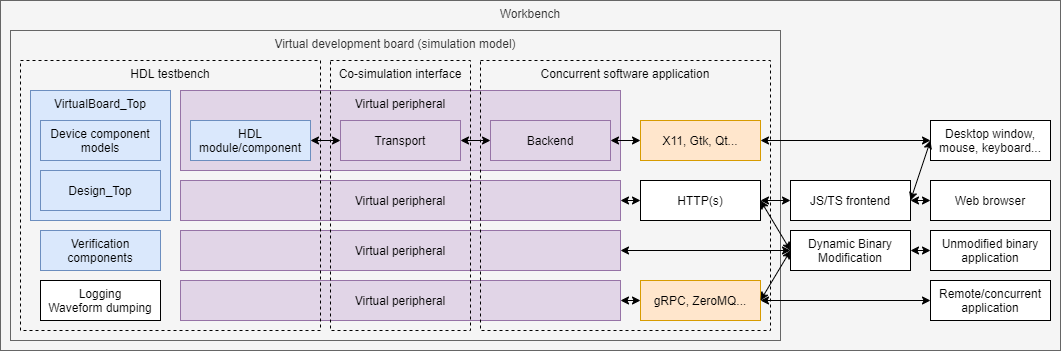
\includegraphics[width=\linewidth]{vboard}
\vfill
\Large \href{https://github.com/dbhi/vboard}{\faGithub~dbhi/vboard}

\href{https://github.com/dbhi/vboard/tree/main/vga}{\faCode~dbhi/vboard: vga}
\vfill
\end{frame}

\begin{frame}
\frametitle{Dynamic Binary Hardware Injection (DBHI)}
\centering
\includegraphics[width=\linewidth]{diagram.pdf}

\vfill
\Large\href{https://dbhi.github.io/}{\faGlobe~dbhi.github.io}
\end{frame}

\begin{frame}
\frametitle{Indirect co-simulation with GHDL: VPI}
\centering
\Large

\href{https://github.com/umarcor/osvb/tree/main/fpconv}{\faCode~umarcor/osvb: fpconv}

\href{https://umarcor.github.io/osvb/notebook/fpconv.html}{\faGlobe~umarcor.github.io/osvb/notebook/fpconv}

\end{frame}

\begin{frame}
\frametitle{Mixed-language co-simulation}

\begin{itemize}
  \item \emph{Verilated} models

    \vfill
    \includegraphics[width=\linewidth]{mixedlanguage}
    \vfill

  \item CXXRTL (Yosys)

    \vfill
    \includegraphics[width=\linewidth]{mixedcxxrtl}
    \vfill
\end{itemize}
\end{frame}

\begin{frame}
  \frametitle{Renode by Antmicro}
  \centering
  \includegraphics[width=\linewidth]{renode.png}

  \vfill
  \Large
  renode.io
  \href{https://renode.io/}{\faGlobe}
  \href{https://docs.google.com/presentation/d/1j0gjI4pVkgF9CWvxaxr5XuCKakEB25YX2n-iFxlYKnE}{\faSlideshare}
\end{frame}

\begin{frame}
\frametitle{Mixed-signal co-simulation}
\centering
\includegraphics[width=.75\linewidth]{xyce}
\vfill
\Large
\href{https://ghdl.github.io/ghdl-cosim/vhpidirect/examples/vffi_user.html\#xyce}{\faGlobe~ghdl-cosim: vhpidirect/examples/vffi\_user/Xyce}
\end{frame}

\begin{frame}
\frametitle{Use cases}
\centering
\includegraphics[width=\linewidth]{usecases}
\end{frame}

\begin{frame}
  \frametitle{Software-Hardware co-design}
  \centering
  \href{https://umarcor.github.io/SIEAV/Co-design.html}{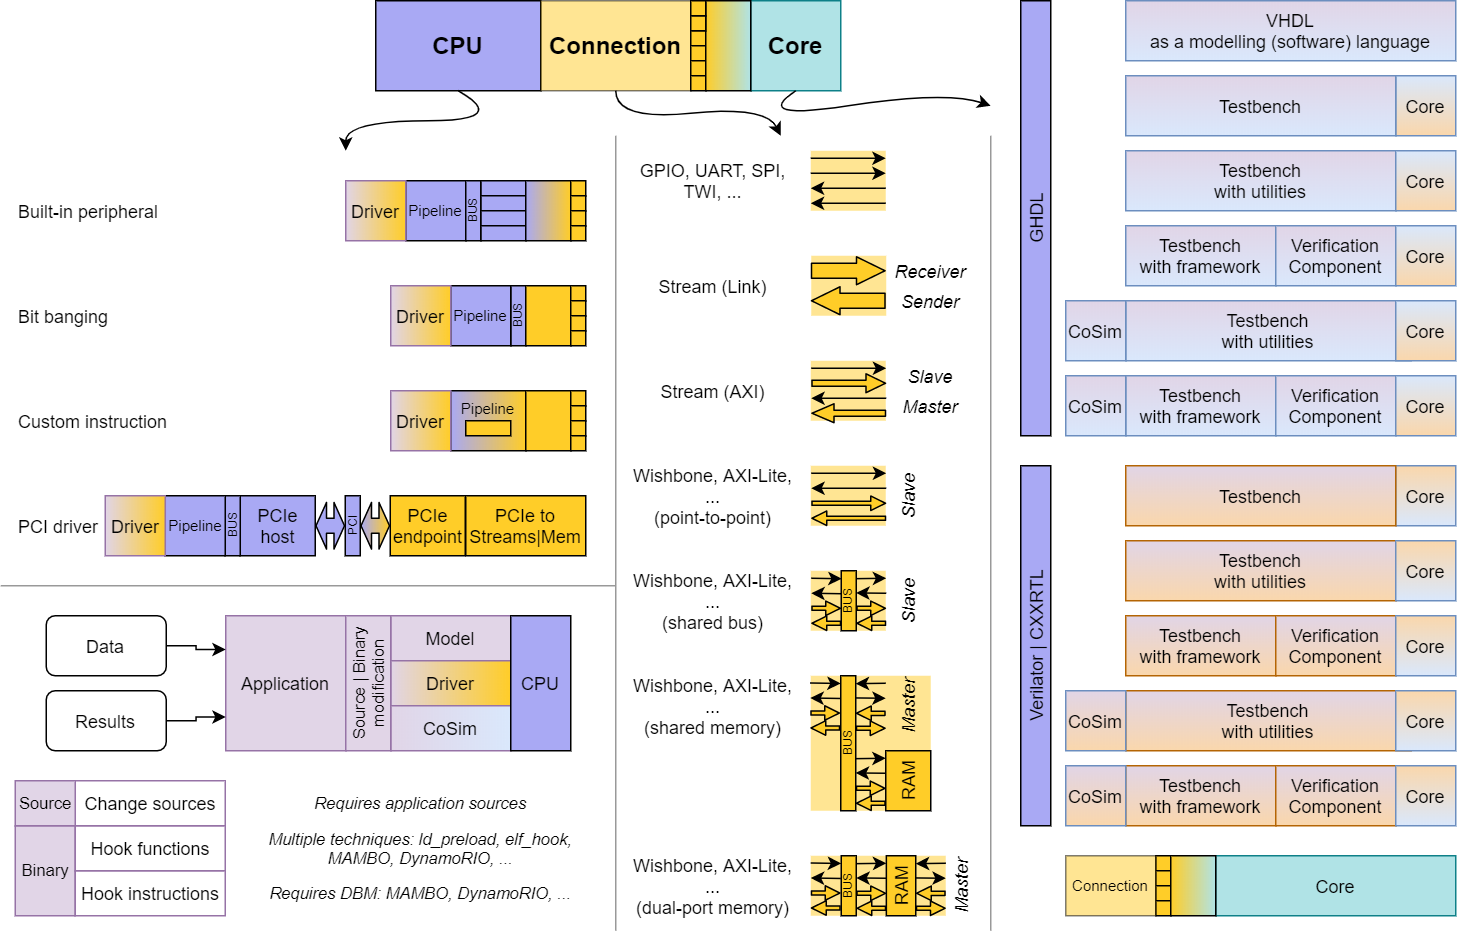
\includegraphics[width=.35\linewidth]{software-hardware}}
  \vfill
  \includegraphics[width=.85\linewidth]{control_socmem.pdf}
\end{frame}

\end{document}
